\section{Analyser les résultats}

\begin{frame}{Classement à budget de temps égal}
  \scriptsize
  \begin{columns}[T,onlytextwidth]
    \begin{column}{0.50\textwidth}
      \renewcommand{\arraystretch}{1.12}
      \setlength{\tabcolsep}{3pt}
      \begin{tabular}{@{}lrr@{}}
        \toprule
        Méthode & Écart & Rang \\
        \midrule
        Recuit simulé & \textbf{0,015} & \textbf{1,25} \\
        Tabou $\times$ Recuit & \textbf{0,018} & 1,75 \\
        Tabou & 0,240 & 3,55 \\
        Génétique $\times$ Tabou & 0,261 & 3,75 \\
        SMA & 1,078 & 5,05 \\
        SMA $\times$ Méta & 1,196 & 6,15 \\
        Génétique $\times$ Recuit & 2,031 & 6,50 \\
        Fourmis $\times$ Tabou & 1\,006,0 & 8,00 \\
        Fourmis (ACO) & 2\,031,2 & 9,00 \\
        Génétique & 2\,836,2 & 10,00 \\
        \bottomrule
      \end{tabular}
    \end{column}

    \begin{column}{0.48\textwidth}
      \centering
      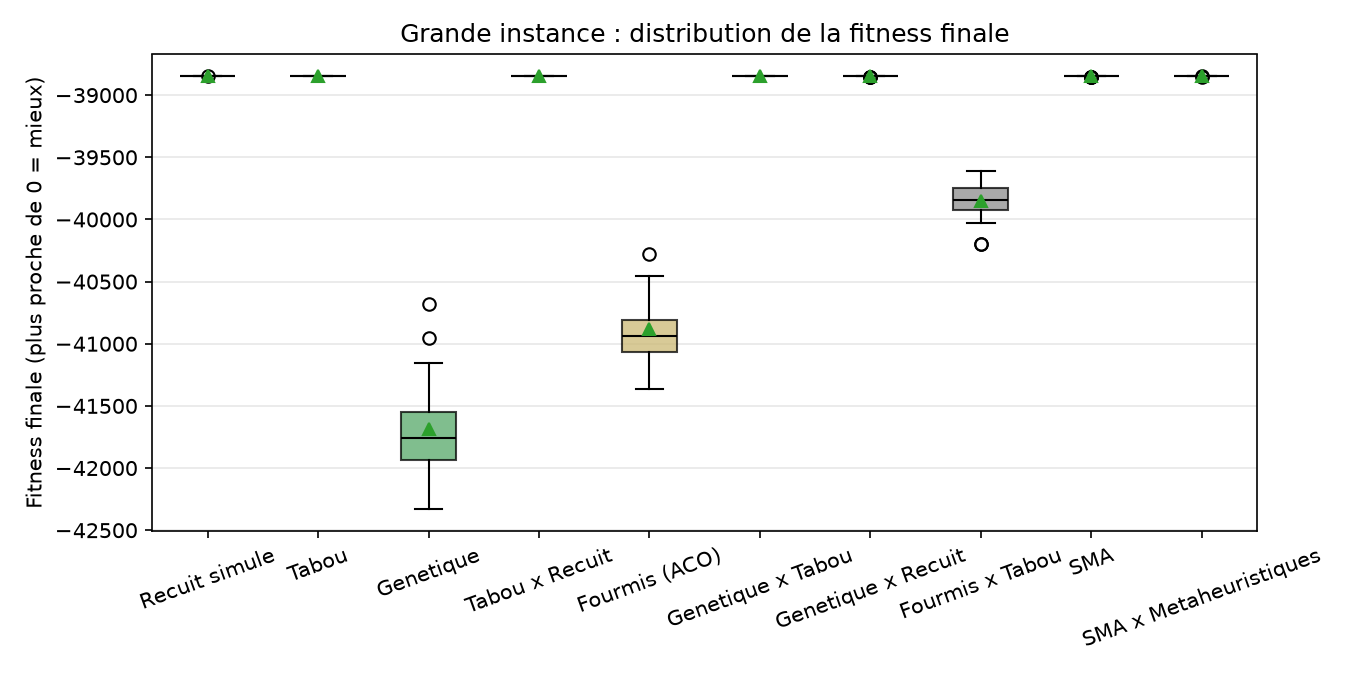
\includegraphics[width=\linewidth,height=0.30\textheight,keepaspectratio]{grande_boxplot.png}
      \credit{Dispersion de la fitness finale, grande échelle.}
      \uncover<2->{\par\vspace{0.12cm}\footnotesize Les méthodes locales
        dominent ; Génétique $\times$ Tabou et Fourmis $\times$ Tabou
        réduisent fortement l'écart. L'écart est mesuré à la meilleure
        solution observée.}
    \end{column}
  \end{columns}
  \source{Campagne \texttt{resultats/benchmark} : 300 patients, 80 vacations,
    20 graines, 3 s ; référence $-38\,847\,195$.}
\end{frame}

\begin{frame}{ML : durée, séjour, ambulatoire}
  \small
  \begin{columns}[T,onlytextwidth]
    \begin{column}{0.48\textwidth}
      \renewcommand{\arraystretch}{1.35}
      \centering
      \begin{tabular}{@{}lrrr@{}}
        \toprule
        Capacité & Médianes & Modèle & Oracle \\
        \midrule
        42 lits & 246 & \textbf{251} & 260 \\
        10 lits & \textbf{111} & 108 & 115 \\
        \bottomrule
      \end{tabular}
      \par\vspace{0.15cm}
      {\footnotesize
        MAE séjour : $1{,}11\rightarrow0{,}44$ jour\\
        F1 ambulatoire : \textbf{0,922}\\
        Intervalle à 90\,\% : $\pm1{,}02$ jour}
    \end{column}

    \begin{column}{0.50\textwidth}
      \footnotesize
      Le gain dépend des ressources.

      \uncover<2->{\par\vspace{0.12cm}À 42 lits, le modèle termine 5
        interventions de plus que les médianes, 9 de moins que l'oracle. À
        10 lits, la capacité sature : la prédiction ne crée pas de place.}
    \end{column}
  \end{columns}
  \source{Cas terminés sur 279, politique réactive, fermeture 10h--12h,
    2 salles, graine 0. Oracle = durées futures révélées, pas optimum
    garanti. Métriques ML : campagne interne de l'équipe.}
\end{frame}

\begin{frame}{SMA : ce que la coordination coûte}
  \small
  \begin{columns}[T,onlytextwidth]
    \begin{column}{0.48\textwidth}
      \renewcommand{\arraystretch}{1.30}
      \centering
      \begin{tabular}{@{}lrr@{}}
        \toprule
        Plan & Terminées / 279 & Dépass. (min) \\
        \midrule
        Figé & 255 & 2\,911 \\
        Réactif & 251 & \textbf{2\,716} \\
        \bottomrule
      \end{tabular}
    \end{column}

    \begin{column}{0.50\textwidth}
      \footnotesize
      Le compromis n'est pas systématique.

      \uncover<2->{\par\vspace{0.12cm}La replanification réduit le
        dépassement de 195 min, mais termine 4 interventions de moins.\par
        \vspace{0.08cm}Rang moyen : 5,05 à 300 patients, 5,85 à 582.\par
        \vspace{0.06cm}La solution reste versionnée et validée avant
        exécution.}
    \end{column}
  \end{columns}
  \source{279 interventions, 42 lits, 2 salles, salle 1 fermée 10h--12h,
    graine 0. Dépassement : occupation et remise en état après 17h.}
\end{frame}
